\documentclass[{../../master}]{subfiles}
\graphicspath{{../../}}  % 個別コンパイル時の画像パスを解決する

\begin{document}

本章ではロボットの動作の制御を行うためのコントローラを作成します.
ロボットのコントローラの構築には,ROSのコントローラフレームワークである\textsf{ros\_control}を使用します.
\textsf{ros\_control}を使うためにはいくつかの準備が必要となるため,結構面倒だったり難しかったりしますが,完成した時の便利さはかなりのものになります.

\section{\textsf{ros\_control}とは}

\textsf{ros\_control}\footnote{\url{http://wiki.ros.org/ros_control}}とは,ロボットのジョイントアクチュエータを制御するためのコントローラインターフェース,コントローラマネージャ,トランスミッション,ハードウェアインターフェース,制御ツールボックスなどを含むパッケージ群のことです.
もともとWillow Garage社のPR2で使用されていたコントローラを一般的なロボットに使用できるように書き直したもので,ロボットに依存しない方法でリアルタイム性能を引き出すコントローラとして開発されました.
\textsf{ros\_control}の枠組みを使用することで,ハードウェアを抽象化してプログラミングを簡単にしたり,共通のコントローラを使って実機のロボットとシミュレーション上のロボットを動かしたりするできるようになります.

\textsf{ros\_control}のシステムの概要図をROS Wikiから引用します.

\begin{figure}[ht]
  \centering
  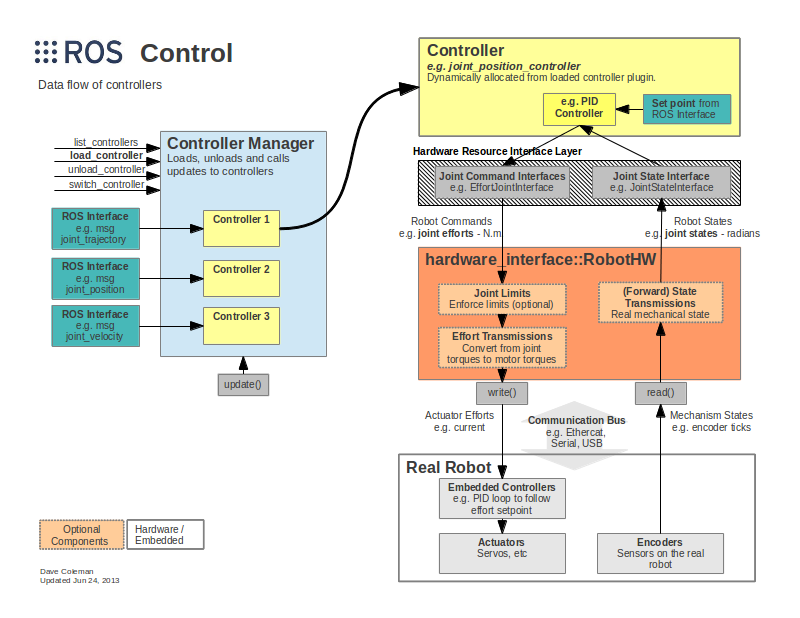
\includegraphics[height=70truemm]{images/ros_control_diagram.png}
  \label{fig:ros_control_diagram}
  \caption{Diagram of \textsf{ros\_control}}
\end{figure}

ADAMR2では,\textsf{ros\_control}に準拠したコントローラである\textsf{diff\_drive\_controller}\footnote{\url{http://wiki.ros.org/diff_drive_controller}}を使用して,ロボットを制御するシステムを構築しています.
次節以降でシステムの構築の手順を説明していきます.

\end{document}